\documentclass{beamer}

\usetheme{Warsaw}

\title{Uppaal. The Model Checker.}
\author{Patryk Kiepas}
\date{\today}

\begin{document}
%-------------------------------------------------------------------------
\begin{frame}
	\titlepage
\end{frame}

%-------------------------------------------------------------------------	
\section*{Outline}
\begin{frame}
	\tableofcontents
\end{frame}

%%%%%%%%%%%%%%%%%%%%%%%%%%%%%%%%%%%%%%%%%%%%%%%%%%%%%%%%%%%%%%%%%%%%%%%%%%
\section{Intro}
%%%%%%%%%%%%%%%%%%%%%%%%%%%%%%%%%%%%%%%%%%%%%%%%%%%%%%%%%%%%%%%%%%%%%%%%%%
\subsection{Quick look}
%-------------------------------------------------------------------------
\begin{frame}{Uppaal. What is it?}
	Uppaal is a model checker for real-time systems (in mind of embedded systems). What we can do with it?
	
	\begin{enumerate}
		\item Modeling
		\item Simulation
		\item Verification
	\end{enumerate}
	
	Internal representation of model consists of:
	
	\begin{itemize}
		\item Network of timed automata
		\item Extended with data types
	\end{itemize}

\end{frame}

\begin{frame}{Where to use?}
	``Any system can be analyzed using a model checker, as long as it has \textit{states} and \textit{transitions} between states'' (from Chapter 1: A First Introduction to Uppaal by Frits Vaandrager) \newline
	
	Reactive systems such as:
	\begin{itemize}
		\item Hardware components
		\item Embedded controllers
		\item Network protocols
		\item Others...
	\end{itemize}
	Whenever there is need to handle real-time issues (the timing of transitions).
	
\end{frame}

\subsection{History}
%-------------------------------------------------------------------------
\begin{frame}{Brief history}
	Uppaal was started by Uppsala University, Sweden and Aalborg University, Denmark.
	
	Timeline of development:
	\begin{itemize}
		\item 1995 - project started
		\item 1999 - first beta
		\item 1999/2000 - first stable release (v 3.0.X)
		\item September 27, 2010 - latest stable release (v 4.0.13)
		\item July 1, 2014 - preview release (v 4.1.19)
	\end{itemize}
	
\end{frame}

\subsection{Versions}
\begin{frame}{Uppaal variations}
	Versions: Windows, Mac, Linux, 32/64 bits
	
	Available licenses:
	\begin{itemize}
		\item Academic use (more info: \href{http://www.uppaal.org/}{http://www.uppaal.org/})
		\item Commercial use (more info: \href{http://www.uppaal.com/}{http://www.uppaal.com/})
	\end{itemize}
\end{frame}

%%%%%%%%%%%%%%%%%%%%%%%%%%%%%%%%%%%%%%%%%%%%%%%%%%%%%%%%%%%%%%%%%%%%%%%%%%	
\section{The tool}
%%%%%%%%%%%%%%%%%%%%%%%%%%%%%%%%%%%%%%%%%%%%%%%%%%%%%%%%%%%%%%%%%%%%%%%%%%
\subsection{Uppaal GUI}
%%%%%%%%%%%%%%%%%%%%%%%%%%%%%%%%%%%%%%%%%%%%%%%%%%%%%%%%%%%%%%%%%%%%%%%%%%
\begin{frame}{Uppaal GUI - Main parts}
\vspace{-10mm}
\begin{columns}
	\begin{column}{0.8\textwidth}
		\begin{figure}[H]
			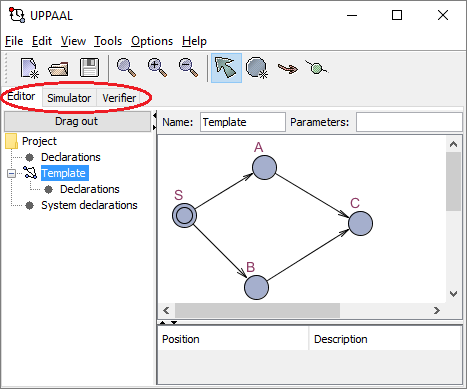
\includegraphics[scale=0.7]{img/uppaal_gui_small_editor.png}
		\end{figure}
	\end{column}
	
	\begin{column}{0.3\textwidth}
		\begin{itemize}
			\item System editor
			\item Simulator
			\item Verifier
		\end{itemize}
	\end{column}
\end{columns}		
\end{frame}

\begin{frame}{Uppaal GUI - System editor}
	\vspace{-10mm}
	\begin{columns}
		\begin{column}{0.8\textwidth}
			\begin{figure}[H]
				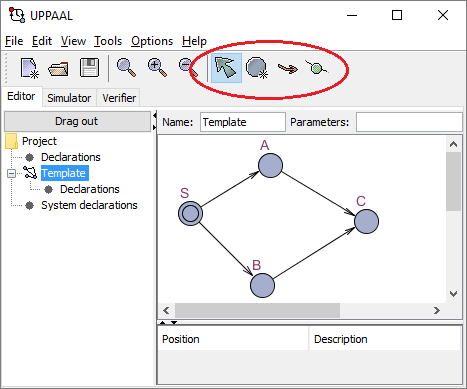
\includegraphics[scale=0.7]{img/uppaal_gui_small_editor_control.png}
			\end{figure}
		\end{column}
		
		\begin{column}{0.3\textwidth}
			\begin{itemize}
				\item Name: Template (defualt)
				\item Select
				\item Add location
				\item Add edge
				\item Add nail
				\item Syntax check (for global, local, system declarations)
			\end{itemize}
		\end{column}
	\end{columns}		
\end{frame}

\begin{frame}{Uppaal GUI - Simulator}
	\vspace{-5mm}
	\begin{columns}
		\begin{column}{0.8\textwidth}
			\begin{figure}[H]
				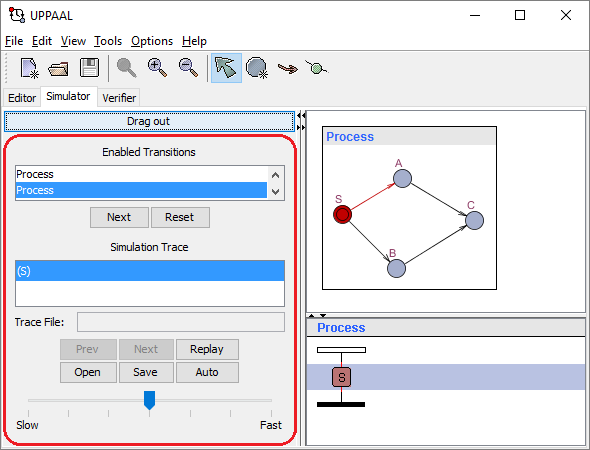
\includegraphics[scale=0.55]{img/uppaal_gui_small_simulation.png}
			\end{figure}
		\end{column}
		
		\begin{column}{0.35\textwidth}
			\begin{itemize}
				\item Select transition
				\item Track simulation
				\item Control (Prev/Next/Auto)
				\item Visualization
			\end{itemize}
		\end{column}
	\end{columns}		
\end{frame}

\begin{frame}{Uppaal GUI - Verifier}
	\vspace{-5mm}
	\begin{columns}
		\begin{column}{0.8\textwidth}
			\begin{figure}[H]
				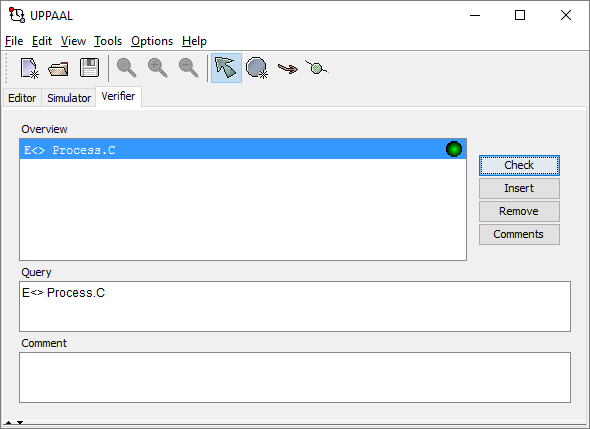
\includegraphics[scale=0.55]{img/uppaal_gui_small_verification.png}
			\end{figure}
		\end{column}
		
		\begin{column}{0.35\textwidth}
			\begin{itemize}
				\item Query editor
				\item Check query
				\item Overview
				\item Save/load
			\end{itemize}
		\end{column}
	\end{columns}		
\end{frame}

%%%%%%%%%%%%%%%%%%%%%%%%%%%%%%%%%%%%%%%%%%%%%%%%%%%%%%%%%%%%%%%%%%%%%%%%%%	
\subsection{Project structure}
%%%%%%%%%%%%%%%%%%%%%%%%%%%%%%%%%%%%%%%%%%%%%%%%%%%%%%%%%%%%%%%%%%%%%%%%%%
\begin{frame}{Project}
	All projects consist of:
		
	\begin{itemize}
		\item Global declaration for whole project
		\item Processes modelled using timed automata
		\item Local declaration for each process
		\item System description
	\end{itemize}
\end{frame}

\begin{frame}{Model/system}
	
	A Uppaal model (called system) is defined as a composition of a number of basic components (called automata or processes). Automata are diagrams with states
	(called locations) and transitions between states (called edges).\newline

\end{frame}

\begin{frame}{Process/automata}
	Each automaton has at most one initial location, marked
	by a double circle.
	
	(!)Deadlock - is when no further transitions are possible and therefore a deadlock state
	has been reached.
\end{frame}

\begin{frame}{Location/state}
	
	If a location is Urgent then this means that time can not elapse within this
	location, and hence a transition to another location will occur immediately.
	
	Each automaton has at most one initial location, marked
	by a double circle.
\end{frame}

\begin{frame}{Parameters}
	
	Parameters can be declared to have either call-by-value or call-by-reference semantics, that is, a template may have access to either a local copy of the argument or to the original. The syntax is taken from C++, where the identifier of a call-by-reference parameter is prefixed with an ampersend in the parameter declaration. Clocks and channels must always be call-by-reference parameters.
	
	
	Uppaal does not allow
	data parameters for synchronization channels.
	
	In template paraemetrs field: urgent chan \&get, chan \&put.
	When creating templates:
	Hammer = Tool(get\_hammer, put\_hammer);
	Mallet = Tool(get\_mallet, put\_mallet);
\end{frame}

\begin{frame}{System declaration}
	
\end{frame}

\begin{frame}{Edge/transition}
	Choices for which the model does not specify how they are resolved are called
	nondeterministic.\newline
	
	Without prior specification, transitions occur instantaneously and do not take time.\newline
	
	Transition have fields:
	\begin{itemize}
		\item Guard
		\item Update
	\end{itemize}
	
	In fields we can declare arrays, Boolean variables, define new ``record'' types and new functions.
	
\end{frame}

\begin{frame}{Channels}
	
	Uppaal does not allow
	data parameters for synchronization channels.
	
	When a synchronization channel is urgent, this means that whenever a synchronization with this channel is enabled, time can not advance and a transition has to be taken immediately.\newline
	
	In order to model the synchronization between tools and jobbers,
	we use the notion of (synchronization) channels from Uppaal. Once “a” has been
	declared as a channel, transitions can be labeled with either a! or a?. This can be
	done by double clicking (within the Editor) transitions with the Select tool, and then
	writing a! or a? in the Sync field. When two automata synchronize on channel “a”,
	this means that an a! transition of one automaton occurs simultaneously with an
	a? transition of another automaton. An a! or a? transition can never occur on its
	own: a! always has to synchronize with a?, and vice versa. If there is one automaton
	S that can do an a! but two automata R1 and R2 that can do an a?, then there is
	a nondeterministic choice and S can synchronize with either R1 or R2. The other
	automaton has do something else or has to wait until the next a! synchronization
	will be offered.
\end{frame}

\begin{frame}{Variables}
	Global/local variables\newline
	
	Examples:\newline
	
	$\text{const int } J = 10;$\\
	$ int[0,J] \text{ jobs}; // \text{ integer with min. value 0 and max. value J}$\newline
	
	The domain of integer is always bounded. By default $int$ has range $[-32768, 32768]$.\newline
	
	Variable assigned with a value outside of its domain generates ``run-time error''.\newline
	
	Transistion can have guards: expressions which use variables. Every transition have guard, by defualt they return \textbf{true}.\newline
	
	Uppaal does not support enumerated types.\newline
	*
	Arrays: const int[0,2] jobs[J] = {H,A,H,H,H,E,E,A,A,A};
\end{frame}

\begin{frame}{Expressions with variables}
	All are C-like:
	\begin{itemize}
		\item jobs++
		\item jobs = jobs + 1
		\item jobs := jobs + 1
	\end{itemize}
	
\end{frame}

\begin{frame}{Time and clocks}
	It allows to track:
	\begin{itemize}
		\item The ordering of events
		\item How fast some events occur
	\end{itemize}
	
	In Uppaal we can specify upper bounds on timing, using so-called “invariants”.
	When we double click the location work easy, a window appears with a field In-variant.
	
	If we want to specify lower and upper bounds on the time that an automaton may
	stay in a certain location, we can do this in Uppaal using so-called clocks. A clock
	is a special type of variable, whose domain consists of the set of nonnegative real
	numbers. Just like other variables, clocks can be declared either as a global variable
	(which can be tested and updated by all automata) or as a local variable (which can
	only be used by one automaton). In the initial state, all clocks have value 0. When
	an automaton is waiting in a location and time elapses then the values of its clocks
	increase. More precisely, when t time units pass then the values of all clocks in the
	model increase with t. Thus, all clocks are “perfect” and increase at exactly the same
	rate as real-time. In reality, of course, no clock is 100% perfect, but in our modeling
	language it is convenient to use the idealization of perfect clocks to specify upper
	and lower bounds on the timing of transitions.
\end{frame}

\begin{frame}{Verification}
	
	Whereas the Verifier has an option to compute the fastest execution leading to
	a certain state, there is no corresponding option to compute the slowest execution.
\end{frame}

\begin{frame}{Queries (part I)}
	Query is a property that may or may not hold for a given model. The Verifier can establish whether a Query is \textbf{satisfied} or \textbf{not}.\newline
	Notation:
	\begin{itemize}
		\item $A[]$ - for all reachable states...
		\item $E<>$ - there exists a reachable state...
	\end{itemize}
	Simple queries are in form of $A[] e$ and $E<> e$ where $e$ is an expression build from \textbf{boolean combination} of \textbf{atomic propositions}.
\end{frame}

\begin{frame}{Queries (part II)}
	Atomic propositions can be of the form $A.c$, for $A$ an automaton and $c$ a location. Such a proposition is true in a global state of the model if in this state automaton $A$ is in location $c$.\newline
	
	\begin{tabular}{|c|c|c|}
		\hline \textbf{Expression} & \textbf{Name} & \textbf{True when...} \\ 
		\hline $e\text{ }\&\&\text{ }f$ & and & $e$ and $f$ evaluate to \textbf{true}	 \\ 
		\hline $e\text{ }||\text{ }f$ & or & $e$ or $f$ evaluate to \textbf{true} \\ 
		\hline $e\text{ }==\text{ }f$ & equality & $e$ and $f$ evaluate to the same value \\ 
		\hline $e\text{ }imply\text{ }f$ & implication & $e$ evaluate to \textbf{false} or $f$ evaluate to \textbf{true}\\ 
		\hline $e\text{ }not\text{ }f$ & negation & $e$ evaluates to \textbf{false} \\ 
		\hline 
	\end{tabular} 

\end{frame}

\begin{frame}{Query examples}
	\begin{itemize}
		\item $A[] \text{ not deadlock}$
		\item $E<> \text{Process\_1.C}$
		\item $E<> (\text{Process\_1.C } \&\& \text{ Process\_2.C})$
		\item $A[] \text{ now } >= \text{ 200 imply }$
		$(\text{Belt.end } \&\& \text{ Jobber1.begin } \&\& \text{Jobber2.begin})$
		
	\end{itemize}
\end{frame}

\begin{frame}{Reasoning}
	(!)The tool just uses brute force to explore all the reachable global states of the model and to check for each of these	states whether both jobbers are working on a hard job.
\end{frame}

\begin{frame}{Diagnostic traces}
	
	(!)Uppaal can also provide a concrete example that illustrates why the property holds (for $E<>$ properties) or not (for $A[]$ properties, so called: \textit{counterexample}).\newline
	
	(!)In the case of $E<>$ properties that do not hold, or $A[]$ properties that hold, Uppaal can only report that it exhaustively checked all the reachable states of the model and didn’t find anything.\newline
	
	(!)We choose under \textit{Options} the entry \textit{Diagnostic Trace} and then select the option \textit{Shortest}. Simulator will then show found diagnostic trace.
\end{frame}

\begin{frame}{Saving data}
	We can save various data:
	
	\begin{itemize}
		\item Model/system - \textit{*.xml} file
		\item Queries - \textit{*.q} file
		\item Traces (binary) - \textit{*.xtr} file
	\end{itemize}
\end{frame}

%%%%%%%%%%%%%%%%%%%%%%%%%%%%%%%%%%%%%%%%%%%%%%%%%%%%%%%%%%%%%%%%%%%%%%%%%%	
\section{Example}
%%%%%%%%%%%%%%%%%%%%%%%%%%%%%%%%%%%%%%%%%%%%%%%%%%%%%%%%%%%%%%%%%%%%%%%%%%

%%%%%%%%%%%%%%%%%%%%%%%%%%%%%%%%%%%%%%%%%%%%%%%%%%%%%%%%%%%%%%%%%%%%%%%%%%	
\section{Bibliography}
%%%%%%%%%%%%%%%%%%%%%%%%%%%%%%%%%%%%%%%%%%%%%%%%%%%%%%%%%%%%%%%%%%%%%%%%%%
\begin{itemize}
	\item F.W. Vaandrager. A First Introduction to Uppaal. In J. Tretmans, editor. Quasimodo Handbook. To appear.
\end{itemize}



\end{document}
